\section{Σύστημα επεξεργασίας δεδομένων}
Ο Ρόλος του Συστήματος επεξεργασίας δεδομένων είναι να πάρει τα ανεπεξέργαστα δεδομένα από την βάση δεδομένων και να δημιουργήσει σχέσεις μεταξύ τους κατηγοριοποιώντας τα. Η Εφαρμογή προσφέρει δεδομένα ανά 4 κατηγορίες, και παράλληλα για κάθε κατηγορία ανά χρονολογική περίοδο. Η κατηγοριοποίηση είναι βασισμένη στα παρακάτω στοιχεία:
\begin{itemize}
    \item Στοιχεία ανά χώρα παραγωγής
    \item Στοιχεία ανά εταιρία παραγωγής
    \item Στοιχεία ανά συντελεστή - ξεχωριστά ανά ηθοποιό, συγγραφέα, σκηνοθέτη και παραγωγό
    \item Στοιχεία ανά είδος ταινίας
\end{itemize}

Η κάθε κατηγορία περιέχει στοιχεία για
την ταινία με την μεγαλύτερή αξιολόγηση, 
την ταινία με την χαμηλότερη αξιολόγηση, 
την μέση βαθμολογία ταινιών για αυτήν την κατηγορία, 
τις ταινίες με τα μεγαλύτερα και τα μικρότερα έσοδα και έξοδα, 
τα μέσα έξοδα / έσοδα ταινιών, 
τον πιο δημοφιλή και λιγότερο δημοφιλή ηθοποιό (ή συμπρωταγωνιστή αν η κατηγορία είναι ανά συντελεστή -- ηθοποιό), 
παραγωγό (η συμπαραγωγό αν η κατηγορία είναι ανά συντελεστή -- παραγωγό), 
σκηνοθέτη (η συν-σκηνοθέτη αν η κατηγορία είναι ανά συντελεστή -- σκηνοθέτη) και 
συγγραφέα (ή συν-συγγραφέα αν η κατηγορία είναι ανά συντελεστή -- συγγραφέα), 
την πιο δημοφιλή και λιγότερο δημοφιλή χώρα παραγωγής (η συμπαραγωγής αν η κατηγορία είναι ανά χώρα παραγωγής), 
την πιο δημοφιλή και λιγότερο δημοφιλή εταιρία παραγωγής (ή συμπαραγωγής αν η κατηγορία είναι ανά εταιρία παραγωγής) κ.α
όπως φαίνονται στο σχήμα ~\ref{model:movieinsights}.

\begin{figure}[p]
    \vspace*{-1cm}
    \hspace*{-1cm}
    \makebox[\linewidth]{
        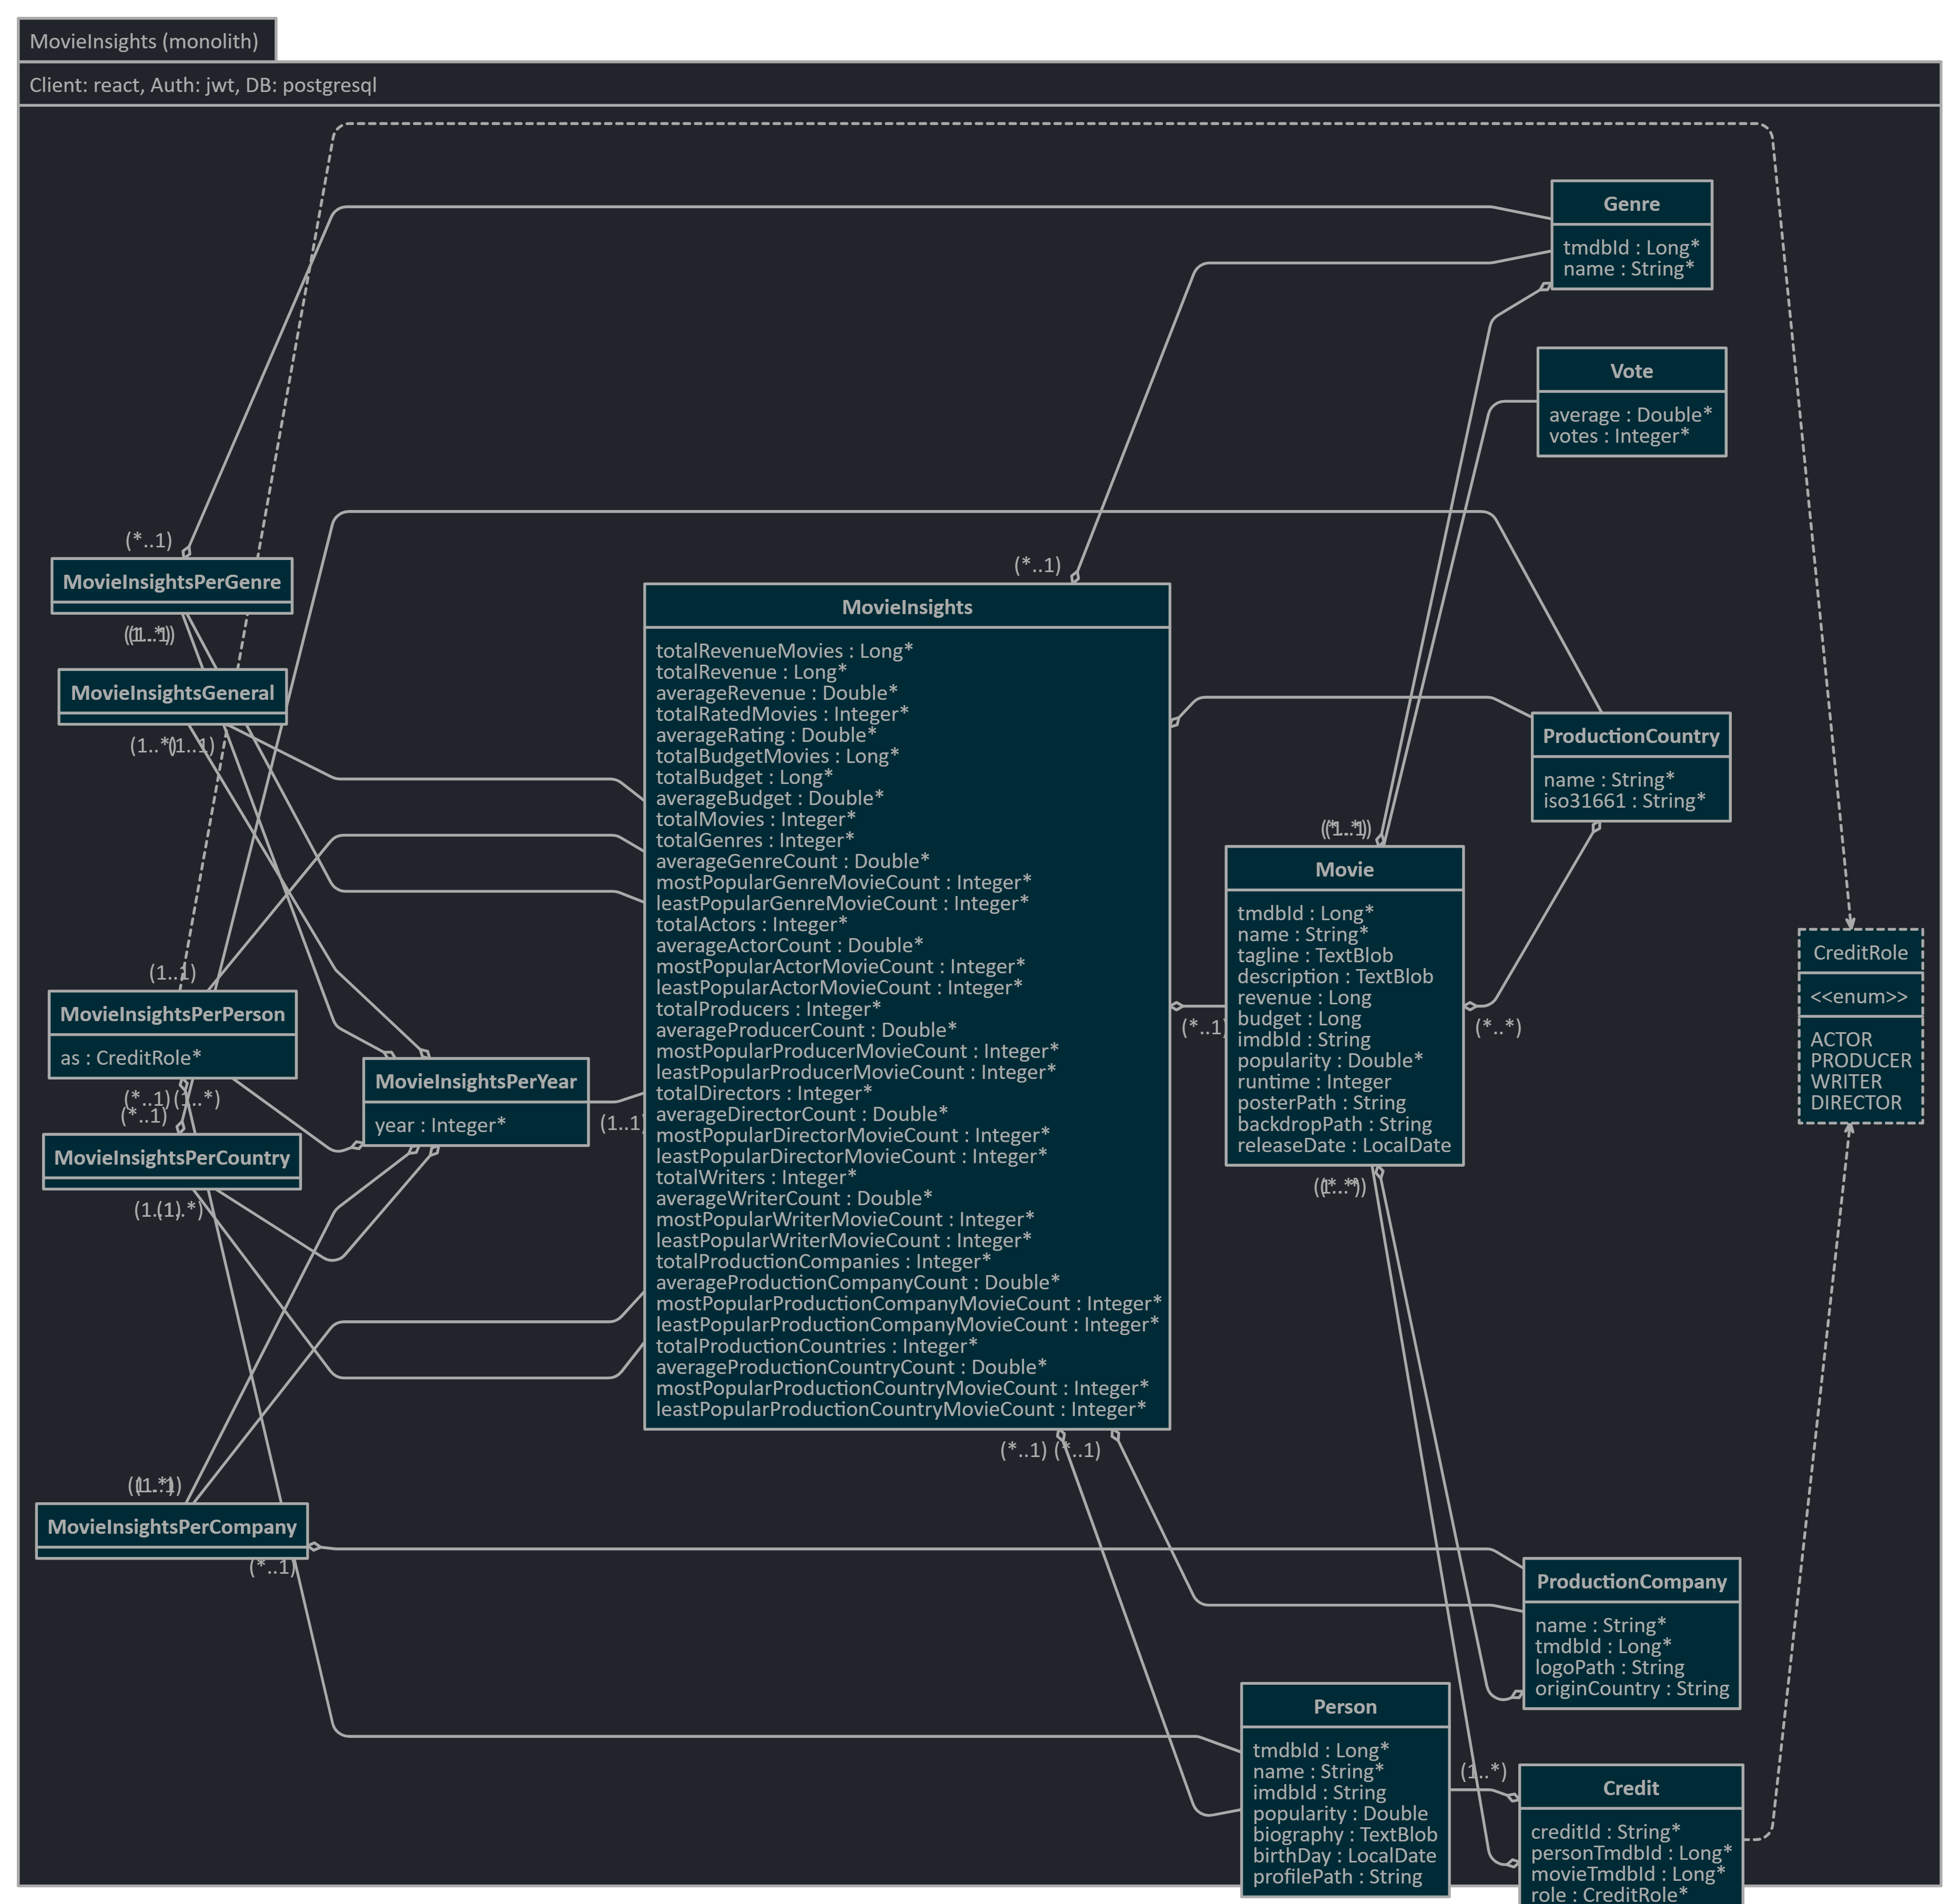
\includegraphics[width=1.4\linewidth]{Chapters/5 - Architecture/MovieInsights/Images/jhipster-jdl (2).png}
    }
   \caption{Μοντελο MovieInsights}
   \label{model:movieinsights}
\end{figure}

Η επεξεργασία των δεδομένων μπορούσε να γίνει είτε στο κομμάτι της βάσης δεδομένων με χρήση της γλώσσας προγραμματισμού SQL είτε στο κομμάτι του Server με χρήση της γλώσσας προγραμματισμού Java. Ο πιο αποδοτικός τρόπος ήταν να γίνει στην βάση δεδομένων με την SQL καθώς υπάρχουν διάφορα συστήματα βελτιστοποίησης τα οποία επιτρέπουν την επεξεργασία των δεδομένων αποδοτικά και γρήγορα, αλλά σε αυτήν την πτυχιακή προτιμήθηκε η Java για λόγους απλότητας.

Το σύστημα επεξεργασίας χωρίζεται σε 3 διαφορετικά κομμάτια. Το πρώτο κομμάτι συλλέγει και κατηγοριοποιεί τα δεδομένα. Το δεύτερο κομμάτι υπολογίζει τα μέγιστα τα ελάχιστα και τους μέσους των δεδομένων. Το τρίτο
κομμάτι μετατρέπει τα δεδομένα σε μια φιλική προς τη βάση δεδομένων μορφή και τα αποθηκεύει.

\subsection{Βήμα 1 - Κατηγοριοποίηση δεδομένων}
\begin{figure}[H]
    \begin{javacode}
    categories = new HashMap<>();
    getMovieInsights(long id, BaseWrapper<?> o) {
        if (categories.containsKey(id)) {
            return categoriess.get(id);
        }
        IMovieInsightsWrapper wrapper = createMovieInsightsWrapper(o);
        categories.put(id,wrapper);
        return wrapper;
    }
    getMovieInsightObjectsOptimized(Movie movie) {
     // return set of getMovieInsights(...)
    }
    categorizeData(Movie movie) {
        Set<IMovieInsightsWrapper> miSet = getMovieInsightObjectsOptimized(movie);
        miSet.forEach(wrapper -> {
            wrapper.submitMovie(movie);
        });
    }
    Lists
      .partition(dto.movies, 1000)
      .forEach(chunk -> {
         chunk.forEach(this::categorizeData);
      });
    \end{javacode}
    \caption{Σειριακή κατηγοριοποίηση με HashMap}
   \label{code:categorieSerialWithHM}
\end{figure}
Ο Αλγόριθμός κατηγοριοποίησης συλλέγει τα δεδομένα, τα προσθέτει στις ανάλογες κατηγορίες, δημιουργεί τις κατηγορίες αν δεν υπάρχουν, και ετοιμάζει τα δεδομένα για τον τελικό υπολογισμό.

Υπήρξαν πολλές αναθεωρήσεις του αλγορίθμου μέχρι την τελική του έκδοση. Οι περισσότερες αφορούσαν βελτιστοποιήσεις απόδοσης. 

Ο Αρχικός κώδικας (βλ σχήμα: \ref{code:categorieSerialWithHM}) ήταν αρκετά απλός. Είχε HashMaps για την αποθήκευση των δεδομένων ανά κατηγορία, και γινόταν συνεχώς έλεγχοι για το αν υπήρχαν τα δεδομένα. Αν όχι τα δημιουργούσε αλλιώς τα μορφοποιούσε.

Αρχικά ο κώδικας έτρεχε σειριακά, καθώς όμως αυξανόταν τα δεδομένα, ανέβαινε εκθετικά και ο χρόνος κατηγοριοποίησης τους. Για παράδειγμα για 1000 ταινίες μαζί με τους συντελεστές, τις εταιρίες και χώρες παραγωγής και τα είδη των ταινιών τους, έκανε 25 λεπτά για την ολοκλήρωση της κατηγοριοποίησης. Για 5000 ταινίες έκανε πάνω από 8 ώρες. 

Ο κώδικας ξαναγράφτηκε (βλ σχήμα: \ref{code:categorieParallelWithCHM}) για να τρέχει με παραλληλισμό. Έτσι κάποια βασικά στοιχεία άλλαξαν, όπως τα HashMaps έγιναν ConcurrentHashMaps και κάποια άλλα κομμάτια έγιναν Synchronize για να υπάρχει Thread Safety. Το αποτέλεσμα αυτών των αλλαγών ήταν η κατηγοριοποίηση 8000 ταινιών, συνυπολογίζοντας και τα λοιπά σχετικά στοιχεία, να ολοκληρώνεται εντός 25 λεπτών.

\begin{figure}[h]
    \begin{javacode}
    categories = new ConcurrentHashMap<>();
    categorizeData(Movie movie) { // ...
        miSet.parallelStream().forEach // ...
    }
    Lists
      // ...
         chunk
            .parallelStream().forEach // ...
      
    \end{javacode}
    \caption{Παράλληλης κατηγοριοποίηση με ConcurrentHashMap}
   \label{code:categorieParallelWithCHM}
\end{figure}

Στην πορεία εμφανίστηκε ένα πρόβλημα απόδοσης, το οποίο δεν ήταν ορατό κατά την πρώτη υλοποίηση, και το οποίο αφορούσε τα HashMaps.
Ενώ δίνουν με μεγάλη ευκολία, είναι στην ουσία ένα Indexer για την αποθήκευση key-value pairs, έχουν μεγάλο performance-pentalty όταν αρχίζει και μεγαλώνει ο όγκος των ανατεθειμένων δεδομένων και το πρόβλημα μεγεθύνεται ακόμα πιο πολύ όταν είναι και ConcurrentHashMaps λόγω των ελέγχων που γίνονται για το Thread Safety. Ένα δείγμα 30000 ταινιών έκανε πάνω από 4.5 ώρες για να κατηγοριοποιήθει.

Κάτι έπρεπε να αντικαταστήσει τα HashMaps. Στην τελική έκδοση του αλγόριθμου (βλ σχήμα: \ref{code:categorieParallelWithArr}) τα HashMaps αντικαταστάθηκαν με τα Native Arrays. Η επιλογή αυτή είχε ιδιαιτέρως θετικό αντίκτυπο στην ταχύτητα της κατηγοριοποίησης αλλά μεγάλωσε η πολυπλοκότητα διαχείρισης των δεδομένων.
Συγκριτικά με τη χρήση ConcurrentHashMaps, όπου η κατηγοριοποίηση 30.000 ταινιών εκτελούνταν σε 4,5 ώρες, ο ανανεωμένος αλγόριθμος κατηγοριοποίησε 30000 ταινίες σε μόλις 8 λεπτά. 

\begin{figure}[h]
    \begin{javacode}
    creditsArray = new MovieInsightsPersonWrapper[dto.maxPersonId][CreditRole.getSize()];
    companiesArray = new MovieInsightsCompanyWrapper[dto.maxCompanyId];
    countriesArray = new MovieInsightsCountryWrapper[dto.maxCountryId];
    genresArray = new MovieInsightsGenreWrapper[dto.maxGenreId];
    
    getMovieInsights(long id, BaseWrapper<?> o, IMovieInsightsWrapper[] array) {
        synchronized (array) {
            IMovieInsightsWrapper wrapper;
            if ((wrapper = array[(int) id]) == null) {
                array[(int) id] = wrapper = createMovieInsightsWrapper(o);
            }
            return wrapper;
        }
    }
    \end{javacode}
    \caption{Παράλληλη κατηγοριοποίηση με Arrays}
   \label{code:categorieParallelWithArr}
\end{figure}
Ο αλγόριθμος λοιπόν κατηγοριοποιεί τα δεδομένα όπως φαίνεται στο σχήμα \ref{flowchart:categorizeData} και αφού τελειώσει προχωράει στο βήμα 2 του υπολογισμού των δεδομένων.
\begin{figure}[H]
  \centering
  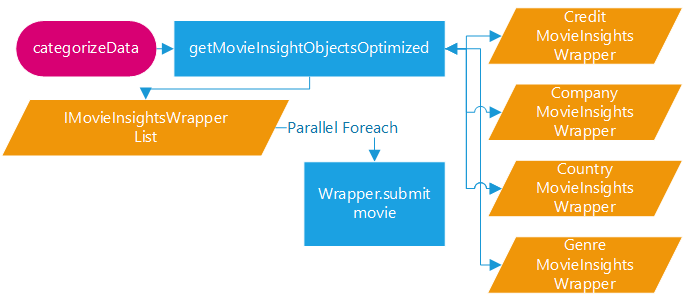
\includegraphics[width=150mm]{Chapters/5 - Architecture/MovieInsights/Images/categorizeData.png}
  \caption{Διάγραμμα ροής κατηγοριοποίησης δεδομένων}
  \label{flowchart:categorizeData}
\end{figure}
\subsection{Βήμα 2 - Υπολογισμός  δεδομένων}

Επιλέγοντας την γλώσσα προγραμματισμού Java για τον υπολογισμό των δεδομένων και επικεντρώνοντας όλες τις βελτιστοποιήσεις στο κομμάτι τις απόδοσης, δημιουργήθηκε ένα νέο πρόβλημα. Επειδή υπάρχουν διπλότυπα δεδομένα λόγω της φύσης της δομής της πτυχιακής, η παρούσα υλοποίηση δεν είναι καθόλου βελτιστοποιημένη για την χρήση μνήμης RAM. Στο πέρας του πρώτο βήματος με δεδομένα 30000 ταινιών κατηγοριοποιημένα, η χρήση μνήμης ξεπερνάει τα 25 GB. Έχοντάς αυτό σαν δεδομένο ο αλγόριθμος υπολογισμού των δεδομένων εκτός από αποδοτικός ως προς την ταχύτητα θα έπρεπε να είναι τουλάχιστον και αποδοτικός ως προς την χρήση μνήμης.

Η αρχική προσέγγιση ήταν ο υπολογισμός των δεδομένων σε κάποια DTO με σκοπό ύστερα την δημιουργία Managed Entities του Hibernate, για να μπορέσουν να αποθηκευτούν στην βάση δεδομένων. Με αυτόν τον τρόπο όμως θα είχαμε ξανά το φαινόμενο των διπλότυπων και θα ξοδεύαμε ακόμα περισσότερη μνήμη καθώς η πλειοψηφία των δεδομένων είναι Native Ints, Longs και Doubles και όχι τόσο Reference Types. Η προσέγγιση που επιλέχτηκε ήταν η δημιουργία ενός Wrapper που κληρονομεί από το Maanaged Entity του Hibernate, κάνοντας και το Wrapper, Managed Entity. Με λίγες ρυθμίσεις πλέον το Wrapper μπορεί να σταλεί απευθείας στον Hibernate για να αποθηκευτεί στην βάση δεδομένων χωρίς να χρειαστεί η δημιουργία κάποιου άλλου Managed Entity.

Για αυτόν τον λόγο ο αλγόριθμος της επεξεργασίας δεδομένων μεταφέρθηκε μέσα σε αυτό το Wrapper έτσι ώστε να μπορεί να τρέξει μετά το πέρας της κατηγοριοποίησης αποδοτικά. Βλέποντας πίσω στο σχήμα(\ref{code:categorieParallelWithCHM}) είναι εμφανές ότι αποστέλλεται μια ταινία στον Wrapper για περαιτέρω επεξεργασία. 

Για να βελτιστοποιηθεί ακόμα περισσότερο στο βήμα της κατηγοριοποίησης ο Wrapper εκτελεί όσους υπολογισμούς μπορεί, που δεν χρειάζονται τα συνολικά δεδομένα για να υπολογιστούν, αλλά μόνο τα υπάρχοντα κάθε φορά σε κάθε submit.

Τα δεδομένα που υπολογίζονται σε κάθε submit είναι οι ταινίες με την μεγαλύτερη και χαμηλότερη βαθμολογία καθώς και η μέση βαθμολογία ταινιών για κάθε κατηγορία και οι ταινίες με τα μεγαλύτερα και χαμηλότερα έσοδα/έξοδα καθώς και τα μέσα έσοδα/έξοδα για κάθε κατηγορία. Τα υπόλοιπα δεδομένα υποβάλλονται και αποθηκεύονται σε HashMaps για τον τελικό υπολογισμό.

Ένα πρόβλημα που αντιμετωπίστηκε στον υπολογισμό της ταινίας με την μεγαλύτερη βαθμολογία ήταν η ακρίβεια της βαθμολογίας. Για παράδειγμα δεν είναι το ίδιο να υπάρχει μια ταινία με βαθμολογία 9.0 και 10.000 ψήφους και μια άλλη ταινία με βαθμολογία 9.0 και 200.000 βαθμολογίες. Όπως επίσης είναι πιο αξιόπιστη μια βαθμολογία για παράδειγμα 8.5 με 2.000.000 ψήφους από ότι μια βαθμολογία 9.0 με 100.000 ψήφους. 

Για την επίλυση αυτού του προβλήματος χρησιμοποιήθηκε ένας πολύ απλός αλγόριθμος βάρους $rating * \log_2(voteCount)$, έτσι ώστε να υπολογίζονται και οι ψήφοι και να βγαίνει ενα "σκορ" ταινίας το οποιο θα συγκρίνεται με τα άλλα "σκορ" ταινιών έτσι ώστε να υπολογίζεται η με μεγαλύτερη ακρίβεια ποια ταινία είχε την μεγαλύτερη βαθμολογία.
\begin{figure}[h]
    \begin{javacode}
double calculateScore(Vote vote, boolean high) {
    return getScore(vote.getAverage(), vote.getVotes(), high, 2);
}
double getScore(double value, double weight, boolean high, int base) {
    double weightLog = Math.log(weight) / Math.log(base);
    return high ? value * weightLog : value / weightLog;
}
    \end{javacode}
    \caption{Αλγόριθμος Βάρους Βαθμολογιών}
   \label{code:logarithmicScore}
\end{figure}

Με τον παραπάνω αλγόριθμο σαν βάση, ο Αλγόριθμος υπολογισμού των ταινιών με την μεγαλύτερη και χαμηλότερη βαθμολογία καθώς και της μέσης βαθμολογίας έχει διαμορφωθεί όπως φαίνεται στο σχήμα ~\ref{code:ratingCalculation}. Αρχικά γίνεται έλεγχος αν οι ψήφοι της βαθμολογίας της εν λόγω ταινίας είναι περισσότεροι ή ίσοι με την τιμή της σταθεράς {\it MINIMUM\_VOTES\_THRESHOLD}. Αν δεν είναι, η ταινία εξαιρείται από αυτόν τον υπολογισμό. Αλλιώς προστίθεται η βαθμολογία της ταινίας σε μια μεταβλητή που κρατάει το άθροισμά όλων των βαθμολογιών και αυξάνεται η μεταβλητή που κρατάει και πόσες ταινίες έχουν υποβάλει τις βαθμολογίες τους, για να υπολογιστεί αργότερα η μέση βαθμολογία ταινιών. Ύστερα αν δεν υπάρχει ήδη ταινία με την μεγαλύτερη η χαμηλότερη βαθμολογία τοποθετείται αυτή για την οποία γίνεται ο έλεγχος αυτήν την χρονική στιγμή, αλλιώς γίνεται έλεγχος αν αυτή η ταινία έχει μεγαλύτερη / μικρότερη βαθμολογία από την ανάλογη υπάρχουσα και ορίζεται αυτή στην θέση της σε περίπτωση που πληροί της προϋποθέσεις.

\begin{figure}[h]
    \begin{javacode}
void submitRating(Movie movie) {
    if (movie.getVote().getVotes() >= Constants.MINIMUM_VOTES_THRESHOLD) {
        synchronized (voteLock) {
            Vote vote = movie.getVote();
            totalVoteAverage += vote.getAverage();
            setTotalRatedMovies(getTotalRatedMovies() + 1);
            if (getHighestRatedMovie() == null) {
                setHighestRatedMovie(movie);
            } else {
                setHighestRatedMovie(calculateVote(calculateScore(getHighestRatedMovie().getVote(), true), getHighestRatedMovie(),calculateScore(movie.getVote(), true),movie,(current, challenger) -> current < challenger));
            }
            if (getLowestRatedMovie() == null) {
                setLowestRatedMovie(movie);
            } else {
                setLowestRatedMovie(calculateVote( getLowestRatedMovie().getVote().getAverage(),getLowestRatedMovie(), movie.getVote().getAverage(),movie,(current, challenger) -> current > challenger));
            }
        }
    }
}   
    \end{javacode}
    \caption{Αλγόριθμος Υπολογισμού Βαθμολογιών}
   \label{code:ratingCalculation}
\end{figure}

Ο υπολογισμοί των ταινιών με τα μεγαλύτερα, μικρότερα και μέσα έσοδα / έξοδα γίνεται με έναν πολύ παρόμοιο τρόπο όπως των βαθμολογιών των ταινιών, χωρίς βέβαια να χρησιμοποιείται ο αλγόριθμος βάρους.

Ο υπολογισμός των υπόλοιπων δεδομένων γίνεται μετά το πέρας του βήματος της κατηγοριοποίησης. Για να γίνει πιο εύκολος ο υπολογισμός, αντί να υποβάλλονται τα δεδομένα ως έχουν έχουν δημιουργηθεί Wrappers γύρο από αυτά για την προσθήκη επιπρόσθετων δεδομένων και λειτουργιών που καθιστούν τον υπολογισμό των δεδομένων πιο εύκολο. Για παράδειγμα ένα αντικείμενο τύπου Genre έχει το ανάλογο GenreWrapper, όπως επίσης και ένα αντικείμενο τύπου Person έχει ανάλογα ActorWrapper, DirectorWrapper, ProducerWrapper και WritterWrapper για κάθε κατηγορία ατόμου που υποστηρίζεται από την εφαρμογή. Σε αυτά τα Wrappers υπάρχουν δεδομένα όπως ο αριθμός ταινιών που συμμετέχουν αυτά τα Wrappers για αυτήν την κατηγορία, οι ταινίες οι ίδιες, και υπάρχουν και λειτουργίες σύγκρισης (Comparators) μεταξύ ίδιων Wrappers χρησιμοποιώντας αυτά τα παραπάνω δεδομένα.

Όταν γίνεται η υποβολή δημιουργείται αρχικά ένα Wrapper προσθέτοντάς μεταδεδομένα χωρίς να ελεγχθεί αν υπάρχει ήδη Wrapper που να αναφέρεται στο ίδιο αντικείμενο, αποθηκευμένο στο ανάλογο HashMap οπως φαίνεται στο σχήμα \ref{code:submitGenre}, στην σειρά 5 για την υποβολή δεδομένων ειδών ταινιών.
\begin{figure}[h]
    \begin{javacode}
void submitGenres(Movie movie) {
    AtomicBoolean hasIncreased = new AtomicBoolean(false);
    movie.getGenres().parallelStream().filter(Objects::nonNull).forEach(genre -> {
        calculateTotals(genreTotals, hasIncreased);
        submit(new GenreWrapper(genre, processor.getMovieCount(genre)), genres, movie, genre);
    });
}
    \end{javacode}
    \caption{Αλγόριθμος Υποβολής Δεδομένων Είδους Ταινίας}
    \label{code:submitGenre}
\end{figure}

Στην γενικευμένη συνάρτηση submit πάραυτα γίνεται εκεί ο έλεγχος για την ύπαρξη του ανάλογου Wrapper, και αν υπάρχει απλά αγνοεί το νέο Wrapper και αλλάζει το υπάρχων χρησιμοποιώντας τα στοιχεία του νεου, αλλιώς τοποθετεί το δημιουργημένο Wrapper στο ανάλογο HashMap όπως φαίνεται στο σχήμα \ref{code:submit}.

\begin{figure}[h]
    \begin{javacode}
<T extends IdentifiedEntity, W extends BaseWrapper<T>> void submit(W wrapper, Map<Long, W> objMap, Movie movie, T obj) {
    W wrapper2;
    synchronized (objMap) {
        if ((wrapper2 = objMap.putIfAbsent(obj.getId(), wrapper)) == null) {
            wrapper2 = wrapper;
        }
    }
    wrapper2.movies.add(movie);
    wrapper2.count++;
}
    \end{javacode}
    \caption{Αλγόριθμος Γενικευμένης υποβολής δεδομένων}
    \label{code:submit}
\end{figure}

Επιπρόσθετα για τον υπολογισμό αυτών των δεδομένων χρησιμοποιείται μια βοηθητική γενικευμένη κλάση Total, η οποία κρατάει τα στοιχεία για τα μέγιστα, ελάχιστα και μέσα αυτών των δεδομένων. 

Μετά το πέρας της συλλογής και της κατηγοριοποίησης των δεδομένων, το κάθε MovieInsights Wrapper ξεχωριστά θα υπολογίσει τα υπόλοιπα δεδομένα για το ίδιο αλλά και για κάθε εξαρτώμενο Wrapper από αυτό, που στην συγκεκριμένη περίπτωση τα εξαρτώμενα Wrappers, είναι οι κατηγορίες ανά χρόνο.

Για κάθε διαφορετικό Wrapper HashMap θα υπολογιστούν τα μέγιστα και τα ελάχιστα χρησιμοποιώντας τις συναρτήσεις σύγκρισης που υπάρχουν μέσα στα Wrappers, και τα δεδομένα που περιέχουν τα μέγιστα και τα ελάχιστα θα υποβληθούν στα αντικείμενα της βοηθητικής κλάσης Total για την ανάκτηση τους αργότερα, όπως φαίνεται στα σχήματα \ref{code:calculateChildInsights} και \ref{code:getWrapperBasedOnComparator}.

\begin{figure}[h]
    \begin{javacode}
<W extends BaseWrapper<WE>, WE> void calculateChildInsights(Map<Long, W> map, Comparator<? super W> comparator, Total<WE> totals) {
    Optional<W> mostPopularEntryResult = getWrapperBasedOnComparator(map, comparator.reversed());
    mostPopularEntryResult.ifPresent(totals::submitMostPopular);
    Optional<W> leastPopularEntryResult = getWrapperBasedOnComparator(map, comparator);
    leastPopularEntryResult.ifPresent(totals::submitLeastPopular);
    totals.setTotalEntities(map.size());
}
    \end{javacode}
    \caption{Γενικευμένος Αλγόριθμος υπολογισμού μέγιστων και ελάχιστων δεδομένων}
    \label{code:calculateChildInsights}
\end{figure}
\begin{figure}[h]
    \begin{javacode}
private <W extends BaseWrapper<EW>, EW> Optional<W> getWrapperBasedOnComparator(Map<Long, W> wrapperMap, Comparator<? super W> comparator) {
    return wrapperMap.values().parallelStream().sorted(comparator).filter(e -> (slave ? master.getCategory() : getCategory()) != e.category || e.object != (slave ? master.getSource().object : source.object)).findFirst();
}
    \end{javacode}
    \caption{Γενικευμένος Αλγόριθμος ανάκτησης Wrapper απο ενα HashMap με βάση αλγόριθμο σύγκρισης}
    \label{code:getWrapperBasedOnComparator}
\end{figure}

Τέλος όλα τα δεδομένα αποθηκεύονται στα πεδία της κληρονομουμένης κλάσης MovieInsights, ανακτώντας τα δεδομένα από τα αντικείμενα της βοηθητικής κλάσης Total.

% \begin{figure}[h]
%     \begin{javacode}
% void submitRevenue(Movie movie) {
%     if (movie.getRevenue() >= Constants.MINIMUM_REVENUE_THRESHOLD) {
%         synchronized (revenueLock) {
%             setTotalRevenue(getTotalRevenue() + movie.getRevenue());
%             setTotalRevenueMovies(getTotalRevenueMovies() + 1);
%             if (getHighestRevenueMovie() == null) {
%                 setHighestRevenueMovie(movie);
%             } else {
%                 if (getHighestRevenueMovie().getRevenue() < movie.getRevenue()) {
%                     setHighestRevenueMovie(movie);
%                 } else if (getHighestRevenueMovie().getRevenue().equals(movie.getRevenue()) && movie.getPopularity() > getHighestRevenueMovie().getPopularity()) {
%                     setHighestRevenueMovie(movie);
%                 }
%             }
%             if (getLowestRevenueMovie() == null) {
%                 setLowestRevenueMovie(movie);
%             } else {
%                 if (getLowestRevenueMovie().getRevenue() > movie.getRevenue()) {
%                     setLowestRevenueMovie(movie);
%                 } else if (getLowestRevenueMovie().getRevenue().equals(movie.getRevenue()) && movie.getPopularity() > getLowestRevenueMovie().getPopularity()) {
%                     setLowestRevenueMovie(movie);
%                 }
%             }
%         }
%     }
% }    
%     \end{javacode}
%     \caption{Αλγόριθμος Υπολογισμού Εσόδων}
%   \label{code:revenueCalculation}
% \end{figure}
% \begin{figure}[h]
%     \begin{javacode}
% void submitBudget(Movie movie) {
%     if (movie.getBudget() >= Constants.MINIMUM_BUDGET_THRESHOLD) {
%         synchronized (budgetLock) {
%             setTotalBudget(getTotalBudget() + movie.getBudget());
%             setTotalBudgetMovies(getTotalBudgetMovies() + 1);
%             if (getHighestBudgetMovie() == null) {
%                 setHighestBudgetMovie(movie);
%             } else {
%                 if (getHighestBudgetMovie().getBudget() < movie.getBudget()) {
%                     setHighestBudgetMovie(movie);
%                 } else if (getHighestBudgetMovie().getBudget().equals(movie.getBudget()) && movie.getPopularity() > getHighestBudgetMovie().getPopularity()) {
%                     setHighestBudgetMovie(movie);
%                 }
%             }
%             if (getLowestBudgetMovie() == null) {
%                 setLowestBudgetMovie(movie);
%             } else {
%                 if (getLowestBudgetMovie().getBudget() > movie.getBudget()) {
%                     setLowestBudgetMovie(movie);
%                 } else if (getLowestBudgetMovie().getBudget().equals(movie.getBudget()) && movie.getPopularity() > getLowestBudgetMovie().getPopularity()) {
%                     setLowestBudgetMovie(movie);
%                 }
%             }
%         }
%     }
% }
%     \end{javacode}
%     \caption{Αλγόριθμος Υπολογισμού Εξόδων}
%     \label{code:budgetCalculation}
% \end{figure}
% \begin{javacode*}{frame=none,fontsize=\small,linenos=false}
% void calculateChildInsights(Map<Long, W> map, Comparator<? super W> comparator, Total<WE> totals)
% \end{javacode*}

\subsection{Βήμα 3 - Αποθήκευση δεδομένων}
Έχοντάς συλλέξει, κατηγοριοποιήσει και υπολογίσει όλα τα απαραίτητα δεδομένα, τα δεδομένα αυτά με ελάχιστες μετατροπές στέλνονται στον Hibernate για να αποθηκευτούν στην βάση δεδομένων έτσι ώστε να τεθεί η εφαρμογή σε κατάσταση ετοιμότητας. 

Για την αποθήκευση δεδομένων δημιουργείται μια νέα "συναλλαγή". Η συναλλαγή αυτή βεβαιώνει ότι αν κάποιο από τα δεδομένα αυτά δεν μπορούσε για οποιονδήποτε λόγω να αποθηκευτεί στην βάση δεδομένων, να ακυρωθεί όλη αυτή η διαδικασία και να τερματίσει η εφαρμογή με το ανάλογο μήνυμα σφάλματος, έτσι ώστε να μπορεί να επιλυθεί απο κάποιον διαχειριστή. Η αποθήκευση μερικών δεδομένων στην βάση δεδομένων θα είχε καταστροφικές συνέπειες στην λειτουργία της εφαρμογής. 

Μετά το πέρας της αποθήκευσης, γίνεται εκκαθάριση του Cache και ζητείται να γίνει και εκκαθάριση μνήμης από τον Garbage Collector το JVM, ώστε να ελευθερωθεί μνήμη για την καλύτερη λειτουργία της εφαρμογής. Πολλές φορές αυτό δεν είναι δυνατό ανάλογα με το JVM που χρησιμοποιείται και έτσι μετά την αρχικοποίηση στην περίπτωση που δεν υπάρχει διαθέσιμη μνήμη συστήνεται η επανεκκίνηση της εφαρμογής.

